\ifdefined\niveldos\else
\documentclass[12pt,letterpaper]{report}
 
%Russian-specific packages
%--------------------------------------
\usepackage[T2A]{fontenc}
\usepackage[utf8]{inputenc}
\usepackage[russian]{babel}
\usepackage[mathscr]{euscript}
\usepackage{mathrsfs}
\usepackage{amsmath,amsthm,amssymb,latexsym,amsfonts}
\usepackage{showkeys}
\usepackage{pythonhighlight}
\usepackage{mdframed}
\usepackage{lipsum}
\usepackage{soul}
\usepackage{amsmath,amssymb}
\usepackage{parskip}
\usepackage{graphicx}
\usepackage{mathtools}
\usepackage[usestackEOL]{stackengine} 
\usepackage{tocloft}
\usepackage{xcolor}
\usepackage{hyperref}
\usepackage{tikz}
\usepackage{thmtools}
\usepackage{amsthm}
\usepackage{mathtools}
\usepackage{pdfcomment}
\usepackage{soul}
\usepackage{blindtext}
\usepackage{todonotes}
\usepackage{authblk}
\graphicspath{ {./images/} }
%%

\DeclarePairedDelimiter\abs{\lvert}{\rvert}%
\DeclarePairedDelimiter\norm{\lVert}{\rVert}%

% Swap the definition of \abs* and \norm*, so that \abs
% and \norm resizes the size of the brackets, and the 
% starred version does not.
\makeatletter
\let\oldabs\abs
\def\abs{\@ifstar{\oldabs}{\oldabs*}}
%
\let\oldnorm\norm
\def\norm{\@ifstar{\oldnorm}{\oldnorm*}}
\makeatother

\newtheorem{theorem}{Предложение}
\newtheorem*{theorem-non}{Предложение}
\newtheorem{lemma}[theorem]{Лемма}
\theoremstyle{definition}
\newtheorem*{conj}{Определение}
\declaretheorem[numbered=no]{definition}

% Definindo novas cores
\definecolor{verde}{rgb}{0.25,0.5,0.35}
\definecolor{jpurple}{rgb}{0.5,0,0.35}
\definecolor{darkgreen}{rgb}{0.0, 0.2, 0.13}
%\definecolor{oldmauve}{rgb}{0.4, 0.19, 0.28}
% Configurando layout para mostrar codigos Java
\usepackage{listings}

\newcommand{\estiloJava}{
\lstset{
    language=Java,
    basicstyle=\ttfamily\small,
    keywordstyle=\color{jpurple}\bfseries,
    stringstyle=\color{red},
    commentstyle=\color{verde},
    morecomment=[s][\color{blue}]{/**}{*/},
    extendedchars=true,
    showspaces=false,
    showstringspaces=false,
    numbers=left,
    numberstyle=\tiny,
    breaklines=true,
    backgroundcolor=\color{cyan!10},
    breakautoindent=true,
    captionpos=b,
    xleftmargin=0pt,
    tabsize=2
}}

\newcommand{\estiloR}{
  \lstset{ %
    language=R,                     % the language of the code
    basicstyle=\footnotesize,       % the size of the fonts that are used for the code
    numbers=left,                   % where to put the line-numbers
    numberstyle=\tiny\color{gray},  % the style that is used for the line-numbers
    stepnumber=1,                   % the step between two line-numbers. If it's 1, each line
                                    % will be numbered
    numbersep=5pt,                  % how far the line-numbers are from the code
    backgroundcolor=\color{white},  % choose the background color. You must add \usepackage{color}
    showspaces=false,               % show spaces adding particular underscores
    showstringspaces=false,         % underline spaces within strings
    showtabs=false,                 % show tabs within strings adding particular underscores
    frame=single,                   % adds a frame around the code
    rulecolor=\color{black},        % if not set, the frame-color may be changed on line-breaks within not-black text (e.g. commens (green here))
    tabsize=2,                      % sets default tabsize to 2 spaces
    captionpos=b,                   % sets the caption-position to bottom
    breaklines=true,                % sets automatic line breaking
    breakatwhitespace=false,        % sets if automatic breaks should only happen at whitespace
    title=\lstname,                 % show the filename of files included with \lstinputlisting;
                                    % also try caption instead of title
    keywordstyle=\color{blue},      % keyword style
    commentstyle=\color{darkgreen},   % comment style
    stringstyle=\color{red},      % string literal style
    escapeinside={\%*}{*)},         % if you want to add a comment within your code
    morekeywords={*,...}          % if you want to add more keywords to the set
}}

\newcommand{\Z}{\mathbb{Z}}
\newcommand{\Q}{\mathbb{Q}}
\newcommand{\N}{\mathbb{N}}
\newcommand{\R}{\mathbb{R}}
\newcommand{\follow}{\textbf{\textit{Следствие:}}}
\newcommand{\notice}{\underline{\textit{Замечание }}}

\newcommand*\circled[1]{\tikz[baseline=(char.base)]{
            \node[shape=circle,draw,inner sep=2pt] (char) {#1};}}

\definecolor{linkcolor}{HTML}{47528f} % цвет ссылок
\definecolor{urlcolor}{HTML}{47528f} % цвет гиперссылок
\hypersetup{pdfstartview=FitH,  linkcolor=linkcolor,urlcolor=urlcolor, colorlinks=true}
\newcommand{\RomanNumeralCaps}[1]
  {\MakeUppercase{\romannumeral #1}}
\usepackage{titlesec}
\renewcommand{\thesection}{\arabic{section}}
\renewcommand{\listtheoremname}{Определения и теоремы}
\renewcommand\qedsymbol{$\blacksquare$}
\newcommand\oast{\stackMath\mathbin{\stackinset{c}{0ex}{c}{0ex}{\ast}{\bigcirc}}}
\makeatletter
\renewenvironment{proof}[1][\proofname]{%
   \par\pushQED{\qed}\normalfont%
   \topsep6\p@\@plus6\p@\relax
   \trivlist\item[\hskip\labelsep\bfseries#1\@addpunct{.}]%
   \ignorespaces
}{%
   \popQED\endtrivlist\@endpefalse
}
\makeatother
%--------------------------------------
\DeclareMathOperator{\Mr}{M_{\mathbb{R}}}
\addtolength{\oddsidemargin}{-.875in}
	\addtolength{\evensidemargin}{-.875in}
	\addtolength{\textwidth}{1.75in}

	\addtolength{\topmargin}{-.875in}
    \addtolength{\textheight}{1.75in}
%--------------------------------------
\def\calloutsym{%
  \ensurestackMath{%
  \scalebox{1.7}{\color{red}\stackunder[0pt]{\bigcirc}{\downarrow}}}%
}
\def\calloutsymup{%
  \ensurestackMath{%
  \scalebox{1.7}{\color{red}\stackon[0pt]{\bigcirc}{\uparrow}}}%
}
\newcommand\callouttext[1]{%
  \def\stacktype{S}\renewcommand\useanchorwidth{T}\stackText%
  \stackunder{\calloutsym}{\scriptsize\Longstack{#1}}\stackMath%
}
\newcommand\callout[3][2.5pt]{%
  \def\stacktype{L}\stackMath\stackunder[#1]{#2}{\callouttext{#3}}%
}
\newcommand\callouttextup[1]{%
  \def\stacktype{S}\renewcommand\useanchorwidth{T}\stackText%
  \stackon{\calloutsymup}{\scriptsize\Longstack{#1}}\stackMath%
}
\newcommand\calloutup[3][1.5pt]{%
  \def\stacktype{L}\stackMath\stackunder[#1]{#2}{\callouttextup{#3}}%
}
%%%%%%%%%%%%%%%%%%%%%%%%%%%%%%%%%%
%                                %
%                                %
%              Title             %
%                                %
%                                %
%%%%%%%%%%%%%%%%%%%%%%%%%%%%%%%%%%
\title{Конспект лекций по математическому анализу

СПбГУ, МКН, 1 курс
\ \\
\ \\ \ \\
} 


%\thanks{Авторы: %\href{https://github.com/maxmartynov08}{maxmart%ynov08}, \href{https://github.com/K-dizzled}{K-%dizzled}, \href{https://github.com/SmnTin}{SmnT%in}, \href{https://github.com/muldrik}{muldrik}%}} 
\author{Лектор: Храбров Александр Игоревич \\
\ \\ \ \\ \ \\ \ \\ \ \\ \ \\ \ \\ \ \\
\ \\ 
\begin{flushright}
Составили: Андрей \href{https://github.com/K-dizzled}{K-dizzled} Козырев \\ Никита  \href{https://github.com/muldrik}{muldrik} Митцев \\ Максим \href{https://github.com/maxmartynov08}{maxmartynov08} Мартынов \\ Семен \href{https://github.com/SmnTin}{SmnTin} Паненков
\end{flushright}
\ \\
\ \\
\ \\
\ \\
\ \\
\ \\}
\date{осень 2020}
\begin{document}

\clearpage
%% temporary titles
% command to provide stretchy vertical space in proportion
\newcommand\nbvspace[1][3]{\vspace*{\stretch{#1}}}
% allow some slack to avoid under/overfull boxes
\newcommand\nbstretchyspace{\spaceskip0.5em plus 0.25em minus 0.25em}
% To improve spacing on titlepages
\newcommand{\nbtitlestretch}{\spaceskip0.6em}
\pagestyle{empty}
\begin{center}
\bfseries
\nbvspace[1]
\Huge
{\nbtitlestretch\huge
КОНСПЕКТ ЛЕКЦИЙ ПО ЛИНЕЙНОЙ АЛГЕБРЕ}

\nbvspace[1]
\normalsize

СПбГУ, МКН, СП, 1 курс\\
ЛЕКТОР: ЖУКОВ ИГОРЬ БОРИСОВИЧ
\nbvspace[1]
\\
\Large СОСТАВИТЕЛИ:\\[0.5em]
\footnotesize АНДРЕЙ \href{https://github.com/K-dizzled}{K-dizzled} КОЗЫРЕВ, НИКИТА  \href{https://github.com/muldrik}{muldrik} МИТЦЕВ \\ МАКСИМ \href{https://github.com/maxmartynov08}{maxmartynov08} МАРТЫНОВ, СЕМЕН \href{https://github.com/SmnTin}{SmnTin} ПАНЕНКОВ

\nbvspace[2]

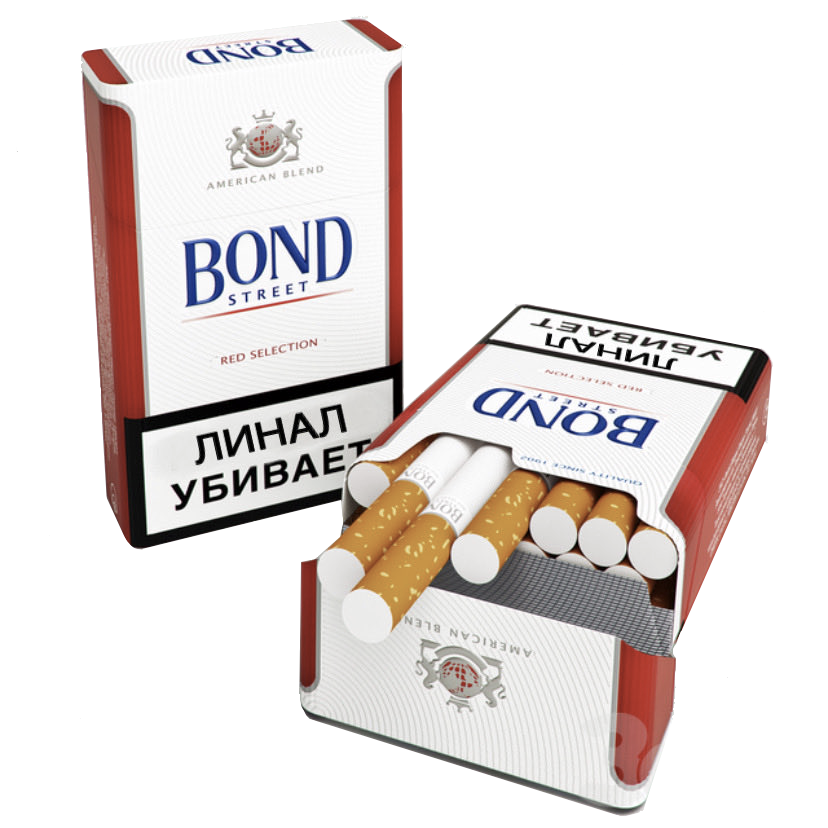
\includegraphics[width=4.0in]{./images/linal_kills.png}
\nbvspace[3]
\normalsize

\large
ОСЕНЬ 2020
\nbvspace[1]
\end{center}
\newpage
\pagestyle{plain}
\fi
%\maketitle
%%%%%%%%%%%%%%%%%%%%%%%%%%%%%%%%%%
%                                %
%                                %
%        Table of content        %
%                                %
%                                %
%%%%%%%%%%%%%%%%%%%%%%%%%%%%%%%%%%
\tableofcontents
%\listoftheorem-nons[ignore={lemma},show={conj, theorem-non}]
% To show Table of contents with
% definitions and lemmas
%----------------------------------------
% \listoftheorem-nons[ignoreall,show={lemma}]
% \listoftheorem-nons[ignoreall,show={conj}]
\newpage
\chapter{Первый семестр. Первая четверть}

\section{Построение поля комплексных чисел.}
\begin{itemize}
  \item $\mathbb{C} = \{a + bi\,|\, a, b \in \mathbb{R} \} \quad i^2 = -1$ 
  \item Определим операцию сложения: $(a + bi) + (a' + b'i) = (a + a') + (b + b')i$
  \item Определеим операцию умножения: $(a + bi) \cdot (a' + b'i) = (aa' - bb') + (ab' + a'b)i$ 
\end{itemize} 
\begin{theorem-non}
  $(\mathbb{C}, +, \cdot)$ - поле
\end{theorem-non}
\begin{proof} \quad \\
  \begin{itemize}
    \item коммутативность и ассоциативность сложения очевидны
    \item $0 + 0i$ - нейтральный по сложению
    \item $(-a) + (-b)i$ - противоположный к $a + bi$
    \item коммутативность умножения очевидна
    \item дистрибутивность умножения:
    \begin{gather*}
      (a + bi)((a_1 + b_1i) + (a_2 + b_2i)) = (a + bi)((a_1 + a_2) + (b_1 + b_2)i) = \\
      = a(a_1 + b_1) - b(b_1 + b_2) + (a(b_1 + b_2) + b(a_1 + a_2))i \\ \\
      (a + bi)(a_1 + b_1i) + (a + bi)(a_2 + b_2i) = (aa_1 - bb_1 + aa_2 - bb_2) + (ab_1 + a_1b + ab_2 + a_2b)i = \\
      = a(a_1 + b_1) - b(b_1 + b_2) + (a(b_1 + b_2) + b(a_1 + a_2))i
    \end{gather*}
    \item ассоциативность умножения:
    \begin{gather*}
      (a_1 + b_1i)((a_2 + b_2i)(a_3 + b_3i)) = (a_1 + b_1i)((a_2a_3 - b_2b_3) + (a_2b_3 + a_3b_2)i) = \\
      = a_1(a_2a_3 - b_2b_3) - b_1(a_2b_3 + a_3b_2) + (a_1(a_2b_3 + a_3b_2) + b_1(a_2a_3 - b_2b_3))i = \\
      = a_1a_2a_3 - a_3b_1b_2 - a_1b_2b_3 - a_2b_1b_3 + (a_1a_2b_3 + a_1a_3b_2 + a_2a_3b_1 - b_1b_2b_3)i  \\ \\
      ((a_1 + b_1i)(a_2 + b_2i))(a_3 + b_3i) = ((a_1a_2 - b_1b_2) + (a_1b_2 + a_2b_1)i)(a_3 + b_3i) = \\
      = (a_1a_2 - b_1b_2)a_3 - (a_1b_2 + a_2b_1)b_3 + ((a_1a_2 - b_1b_2)b_3 + (a_1b_2 + a_2b_1)a_3)i = \\
      = a_1a_2a_3 - a_3b_1b_2 - a_1b_2b_3 - a_2b_1b_3 + (a_1a_2b_3 + a_1a_3b_2 + a_2a_3b_1 - b_1b_2b_3)i
    \end{gather*}
    \item $(1 + 0i)$ - нейтральный элемент по умножению 
    \item $(a + bi)^{-1} = \frac{a}{a^2 + b^2} - \frac{b}{a^2 + b^2}i$
    \begin{gather*}
      (a + bi)(a - bi) = a^2 - b^2i^2 = a^2 + b^2 \quad  /(a^2 + b^2) \\
      (a + bi)(\frac{a}{a^2 + b^2} - \frac{b}{a^2 + b^2}i) = 1
    \end{gather*}
  \end{itemize}
  $\Rightarrow$ все аксиомы поля выполнены $\Rightarrow \mathbb{C}$ - поле комплексных чисел 
\end{proof}
\begin{itemize}
  \item $\mathbb{R}$ это подполе в $\mathbb{C}$ 
  \item $z = x + iy,\; x, y \in \mathbb{R}$ \\
  $x = Re\,z$ - вещественная часть \\
  $y = Im\,z$ - мнимая часть
  \item $z$ называется чисто мнимым, если $Re\,z = 0$
\end{itemize}

\section{Комплексное сопряжение.}
$a - bi$ - число, комплексно сопряженное к $a + bi$
\begin{theorem-non}
  Отображение $\mathbb{C} \to \mathbb{C} : z = x + iy \mapsto \overline{z} = x - yi$ - автоморфизм $\mathbb{C}$, \\
  то есть это биекция, а также $\overline{z_1 + z_2} = \overline{z_1} + \overline{z_2}$ и $\overline{z_1z_2} = \overline{z_1} \cdot \overline{z_2}$
\end{theorem-non}
\begin{proof}
  \begin{enumerate}
    \item $\overline{\overline{x}} = x \Rightarrow$ комплексное сопряжение - отображение, обратное к самому себе $\Rightarrow$ это биекция
    \item  $z_1 = x_1 + iy_1,\; z_2 = x_2 + iy_2$ 
    
    $\overline{z_1 + z_2} = (x_1 + x_2) - (y_1 + y_2)i = (x_1 - y_1i) + (x_2 - y_2i) = \overline{z_1} + \overline{z_2}$
    \item $\overline{z_1z_2} = (x_1x_2 - y_1y_2) - (x_1y_2 + x_2y_1)i$
    
    $\overline{z_1} \cdot \overline{z_2} = (x_1 - y_1i)(x_2 - y_2i) = (x_1x_2 - y_1y_2) - (x_1y_2 + x_2y_1)i$
  \end{enumerate}
\end{proof}
\begin{notice}
  \begin{enumerate}
    \item $z = \overline{z} \Leftrightarrow z \in \mathbb{R}$
    \item $z + \overline{z} \in \mathbb{R}$
    \item $z \cdot \overline{z} \in \mathbb{R}$
  \end{enumerate}
\end{notice}

\section{Определение модуля и аргумента. Свойства модуля комплексного числа.}
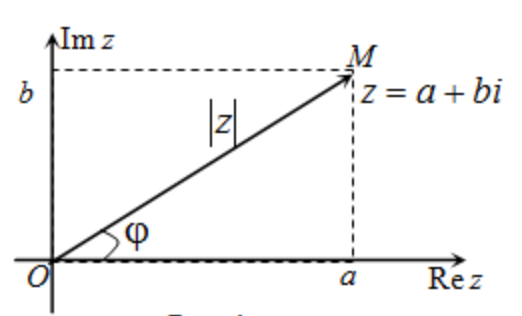
\includegraphics[scale=0.75]{Complex_number_on_plane.png} 
\begin{conj}
  Модулем комплексного числа $z = a + bi$ называется $|z| = \sqrt{a^2 + b^2}$.
\end{conj}
\begin{conj}
  Пусть $z \in \mathbb{C}$, $r = |z|$. Число $\varphi \in \mathbb{R}$ называется аргументом $z$, если 
  \[ z = r(\cos\varphi + i\sin\varphi) \]
\end{conj}
\begin{conj}
  $ z = r(\cos\varphi + i\sin\varphi)$ - тригонометрическая форма комплексного числа.
\end{conj}
\underline{Свойства модуля:}
\begin{enumerate}
  \item $|z| \geqslant 0$ и $|z| = 0 \Leftrightarrow z = 0$
  \item $|\overline{z}| = |z|$
  \item $|z|^2 = z \cdot \overline{z}$
  \begin{proof}
    $z \cdot \overline{z} = (a + bi)(a - bi) = a^2 + b^2 = |z|^2$
  \end{proof}
  \item $|z_1 + z_2| \leqslant |z_1| + |z_2|$
  \begin{proof}
    Будем сравнивать квадраты левой и правой части:
    \begin{gather*}
      |z_1 + z_2|^2 = |(a_1 + a_2) + (b_1 + b_2)i|^2 = (a_1 + a_2)^2 + (b_1 + b_2)^2 = a_1^2 + 2a_1a_2 + a_2^2 + b_1^2 + 2b_1b_2 + b_2^2 \\
      (|z_1| + |z_2|)^2 = a_1^2 + b_1^2 + 2|z_1||z_2|  + a_2^2 + b_2^2 \\
      \Longrightarrow |z_1 + z_2| \leqslant |z_1| + |z_2| \Leftrightarrow a_1a_2 + b_1b_2 \leqslant |z_1||z_2| \\
    \end{gather*}
    Опять возведем левую и правую часть в квадрат:
    \begin{gather*}
      (a_1a_2 + b_1b_2)^2 \leqslant (a_1^2 + b_1^2)(a_2^2 + b_2^2) \\
      2a_1a_2b_1b_2 \leqslant a_1^2b_2^2 + a_2^2b_1^2 \\
      0 \leqslant (a_1b_2 - a_2b_1)^2
    \end{gather*}
  \end{proof}
  \item $|z_1z_2| = |z_1||z_2|$
  \begin{proof}
    Возведем левую и правую часть в квадрат:
    \begin{gather*}
      |z_1z_2|^2 = |(a_1a_2 - b_1b_2) + (a_1b_2 + a_2b_1)i|^2 = (a_1a_2 - b_1b_2)^2 + (a_1b_2 + a_2b_1)^2 = a_1^2a_2^2 + b_1^2b_2^2 + a_1^2b_2^2 + a_2^2b_1^2 \\
      |z_1|^2|z_2|^2 = (a_1^2 + b_1^2)(a_2^2 + b_2^2) = a_1^2a_2^2 + b_1^2b_2^2 + a_1^2b_2^2 + a_2^2b_1^2
    \end{gather*}
  \end{proof}
\end{enumerate}

\section{Существование и «единственность» аргумента комплексного числа. Свойства аргумента.}
\begin{enumerate}
  \item Если $z = 0$, то любое число является его аргументом.
  \item Если $z \neq 0$, то существует $\varphi_0 \in \mathbb{R}$ такое, что $\varphi_0$ - аргумент $z$, и при этом $\varphi_0 + 2\pi k$ для любого $k \in \mathbb{Z}$ тоже аргумент $z$.
  \begin{proof} 
    \begin{gather*}
      x^2 \leqslant x^2 + y^2 = r^2 \Rightarrow -r \leqslant x \leqslant r \\
      -1 \leqslant \frac{x}{r} \leqslant 1 \\
      \Rightarrow \exists\, \widetilde{\varphi} \in \mathbb{R} : \cos\widetilde{\varphi} = \frac{x}{r} \\
      (\sin\widetilde{\varphi})^2 = 1 - (cos\widetilde{\varphi})^2 = 1 - \frac{x^2}{r^2} = \frac{r^2 - x^2}{r^2} = \frac{y^2}{r^2} \\
      \sin\widetilde{\varphi} = \pm\frac{y}{r}
    \end{gather*}
    Если $\sin\widetilde{\varphi} = \frac{y}{r}$, то $\varphi_0 := \widetilde{\varphi}$, иначе $\varphi_0 := -\widetilde{\varphi}$.

    Итого получаем:
    \begin{gather*}
      \cos\varphi_0 = \frac{x}{r} \quad\quad \sin\varphi_0 = \frac{y}{r} \\
      \Rightarrow z = x + iy = r\cos\varphi_0 + r\sin\varphi_0i = r(\cos\varphi_0 + i\sin\varphi_0) \Rightarrow \varphi_0 - arg\,z
    \end{gather*}
    Покажем, что $\varphi = \varphi_0 + 2\pi k$ тоже является аргументом:
    \[ \varphi = \varphi_0 + 2\pi k \Leftrightarrow \cos\varphi = \cos\varphi_0,\, \sin\varphi = \sin\varphi_0 \Leftrightarrow \varphi - arg\,z \]
    Покажем, что все аргументы имеют вид $\varphi_0 + 2\pi k$. Для этого рассмотрим $\alpha \neq (\varphi_0 + 2\pi k)$. 
    Очевидно, что $\cos\alpha \neq \cos\varphi_0$ или $\sin\alpha \neq \sin\varphi_0$. Тогда $r * \cos\alpha \neq x$ или $r * \sin\alpha \neq y$. 
    Следовательно $r(\cos\alpha + i\sin\alpha) \neq z$.
  \end{proof}
\end{enumerate}
\underline{Свойства аргумента:}  

$z_1,\, z_2 \in \mathbb{C}^*$($\mathbb{C}$ без нуля)
\begin{enumerate}
  \item $arg\,z_1z_2 = arg\,z_1 + arg\,z_2$
  \begin{proof}
    \begin{gather*}
      z_1 \cdot z_2 = |z_1|(\cos\varphi_1 + i\sin\varphi_1) \cdot |z_2|(\cos\varphi_2 + i\sin\varphi_2) =  \\
      = |z_1||z_2|(\cos\varphi_1\cos\varphi_2 - \sin\varphi_1\sin\varphi_2 + i(\cos\varphi_1\sin\varphi_2 + \sin\varphi_1\cos\varphi_2)) = \\
      = |z_1||z_2|(\cos(\varphi_1 + \varphi_2) + i\sin(\varphi_1 + \varphi_2))
    \end{gather*}
  \end{proof}
  \item $arg\,\frac{z_1}{z_2} = arg\,z_1 - arg\,z_2$
  \begin{proof}  
      \[ z_1 = \frac{z_1}{z_2} \cdot z_2 \Rightarrow arg\,z_1 = arg\,\frac{z_1}{z_2} + arg\,z_2 \Rightarrow arg\,\frac{z_1}{z_2} = arg\,z_1 - arg\,z_2 \]
  \end{proof}
  \begin{notice}
    $arg\,\frac{1}{z} = arg\,1 - arg\,z = 0 - \arg\,z = -arg\,z$
  \end{notice}
  \item $arg\,\overline{z} = -arg\,z$
  \begin{proof}
    \begin{gather*}
      arg\,z = \varphi \\
      z = |z|(\cos\varphi + i\sin\varphi) \\
      \overline{z} = |z|(\cos\varphi - i\sin\varphi) = |\overline{z}|(\cos(-\varphi) + i\sin(-\varphi)) \\
      \Rightarrow arg\,\overline{z} = -arg\,z
    \end{gather*}
  \end{proof}
\end{enumerate}

\section{Умножение и деление чисел в тригонометрической форме. Формула Муавра.}
\begin{itemize}
  \item \textbf{Умножение} 
  
  $z_1,\, z_2 \in \mathbb{C}^*$
  \[ z_1 \cdot z_2 = |z_1||z_2|(\cos(\varphi_1 + \varphi_2) + i\sin(\varphi_1 + \varphi_2)) \]
  Доказательсво написано выше.
  \item \textbf{Деление} 

  $z_1,\, z_2 \in \mathbb{C}^*$
  \begin{gather*}
    \frac{z_1}{z_2} = \frac{|z_1|(\cos\varphi_1 + i\sin\varphi_1)}{|z_2|(\cos\varphi_2 + i\sin\varphi_2)} = \frac{|z_1|(\cos\varphi_1 + i\sin\varphi_1)(\cos\varphi_2 - i\sin\varphi_2)}{|z_2|(\cos\varphi_2 + i\sin\varphi_2)(\cos\varphi_2 - i\sin\varphi_2)} = \\
    = \frac{|z_1|(\cos\varphi_1\cos\varphi_2 + \sin\varphi_1\sin\varphi_2 + i(\sin\varphi_1\cos\varphi_2 - \cos\varphi_1\sin\varphi_2))}{|z_2|(\cos\varphi_2^2 + \sin\varphi_2^2)} = \\
    = \frac{|z_1|}{|z_2|}(\cos(\varphi_1 - \varphi_2) + i\sin(\varphi_1 - \varphi_2))
  \end{gather*}
  \item \textbf{Формула Муавра}
  
  Пусть $z \in \mathbb{C}^*,\; z = |z|(\cos\varphi + i\sin\varphi)$. 

  Тогда для любого $n \in \mathbb{Z}$
  \[ z^n = |z|^n(\cos(n\varphi) + i\sin(n\varphi)) \]
  \begin{proof} \quad
    \begin{itemize}
      \item $n > 0$
      
      \underline{Индукция по $n$.}

      База $n = 1$: очевидно

      Переход $n = k - 1 \to n = k$
      \begin{gather*}
        z^k = z^{k-1} \cdot z = |z|^{k-1}(\cos(k - 1)\varphi + i\sin(k - 1)\varphi) \cdot |z|(\cos\varphi + i\sin\varphi) =  \\
        = |z|^k(\cos k\varphi + i\sin k\varphi)    
      \end{gather*}
      \item $n = 0$
      
      \[ z^0 = |z|^0(\cos 0 + i\sin 0) = 1 \]
      \item $n < 0$
      \begin{gather*}
        z^n = \frac{1}{z^{-n}} = \frac{1}{|z|^{-n}(\cos(-n\varphi) + i\sin(-n\varphi))} = \\
        = \frac{1}{|z|^{-n}}(\cos(0 - (-n\varphi)) + i\sin(0 - (-n\varphi))) = |z|^n(\cos n\varphi + i\sin n\varphi)
      \end{gather*}
    \end{itemize}
  \end{proof}
  
\end{itemize}



\ifdefined\niveldos\else
\end{document} 
\fi